\documentclass[10pt,a4paper]{article}
\usepackage{amsmath,amssymb,amsthm,graphicx}
\newif\iflipics\lipicsfalse
\usepackage{amsmath}
\usepackage{amsfonts}
\usepackage{amssymb}
\usepackage{amsthm}
\usepackage{xspace}
\usepackage[dvipsnames]{xcolor}
\usepackage{tabularx}
\usepackage{ragged2e}
\usepackage{nicefrac}
\usepackage{bbm}
\usepackage{caption}
\usepackage{graphicx}
\usepackage{enumitem}
\usepackage{soul}
\usepackage{hyperref}
\definecolor{darkgreen}{rgb}{0,0.4,0}
\usepackage{algorithm}
\usepackage[commentColor=darkgreen]{algpseudocodex}
\newcommand{\LineComment}{\LComment}
% \algrenewcomment[1]{\hfill \textit{\textcolor{darkgreen}{$\triangleright$ #1}}}
% \algnewcommand{\LineComment}[1]{\State \textit{\textcolor{darkgreen}{$\triangleright$ #1}}}
\algnewcommand{\IfThenElse}[3]{% \IfThenElse{<if>}{<then>}{<else>}
  \State \algorithmicif\ #1\ \algorithmicthen\ #2\ \algorithmicelse\ #3}
\algdef{SE}[SUBALG]{Indent}{EndIndent}{}{\algorithmicend\ }%
\makeatletter
\renewcommand{\ALG@name}{Listing}
\makeatother
\usepackage{cleveref}
\crefname{listing}{listing}{listings}
\crefname{equation}{eq.}{eqs.}

% must be after cleveref
\newtheorem{theorem}{Theorem}[section]
\newtheorem{lemma}[theorem]{Lemma}
\newtheorem{corollary}[theorem]{Corollary}
\newtheorem{fact}{Fact}[section]
\newtheorem{conj}[theorem]{Conjecture}
\newtheorem{question}[theorem]{Question}
\newtheorem{claim}[theorem]{Claim}
\newtheorem{obs}[theorem]{Observation}
\newtheorem{proposition}[theorem]{Proposition}
\theoremstyle{definition}
\newtheorem{definition}[theorem]{Definition}
\newtheorem{example}{Example}
\newtheorem{results}{Result Family}
\newtheorem{result}{Result}
\theoremstyle{remark}
\newtheorem*{remark}{Remark}
\makeatletter
\newcommand\squeezepar{\@startsection{paragraph}{4}%
{\z@}{1.5ex \@plus1ex \@minus.2ex}{-1em}{\normalfont\normalsize\bfseries}}
\newcommand{\mypara}[1]{\squeezepar{{#1}.}}
\renewcommand{\paragraph}[1]{\squeezepar{{#1}.}}
\makeatother
\graphicspath{{items/}{./}}
\newcommand{\EE}{\mathbb{E}}
\newcommand{\FF}{\mathbb{F}}
\newcommand{\NN}{\mathbb{N}}
\newcommand{\RR}{\mathbb{R}}
\newcommand{\ZZ}{\mathbb{Z}}
\newcommand{\indic}{\mathbbm{1}}
\newcommand{\cA}{\mathcal{A}}
\newcommand{\cB}{\mathcal{B}}
\newcommand{\cC}{\mathcal{C}}
\newcommand{\cD}{\mathcal{D}}
\newcommand{\cE}{\mathcal{E}}
\newcommand{\cF}{\mathcal{F}}
\newcommand{\cG}{\mathcal{G}}
\newcommand{\cH}{\mathcal{H}}
\newcommand{\cI}{\mathcal{I}}
\newcommand{\cJ}{\mathcal{J}}
\newcommand{\cM}{\mathcal{M}}
\newcommand{\cO}{\mathcal{O}}
\newcommand{\cP}{\mathcal{P}}
\newcommand{\cQ}{\mathcal{Q}}
\newcommand{\cR}{\mathcal{R}}
\newcommand{\cS}{\mathcal{S}}
\newcommand{\cU}{\mathcal{U}}
\newcommand{\cV}{\mathcal{V}}
\newcommand{\cW}{\mathcal{W}}
\newcommand{\cX}{\mathcal{X}}
\newcommand{\cY}{\mathcal{Y}}
\newcommand{\cZ}{\mathcal{Z}}

\newcommand{\tG}{\widetilde{G}}
\newcommand{\tS}{\widetilde{S}}
\newcommand{\tO}{\widetilde{O}}
\newcommand{\tP}{\widetilde{P}}
\newcommand{\tQ}{\widetilde{Q}}
\newcommand{\tf}{\widetilde{f}}
\newcommand{\tTheta}{\widetilde{\Theta}}
\newcommand{\tOmega}{\widetilde{\Omega}}
\newcommand{\tM}{\widetilde{M}}
\newcommand{\tmu}{\widetilde{\mu}}

\newcommand{\hw}{\hat{w}}
\newcommand{\hb}{\hat{b}}
\newcommand{\hP}{\hat{P}}
\newcommand{\hf}{\hat{f}}
\newcommand{\hQ}{\hat{Q}}

\newcommand{\ceil}[1]{{\left\lceil{#1}\right\rceil}}
\newcommand{\floor}[1]{{\left\lfloor{#1}\right\rfloor}}
\newcommand{\norm}[1]{{\left\Vert{#1}\right\Vert}}
\DeclareSymbolFont{newfont}{OML}{cmm}{m}{it}% Computer Modern math font
\DeclareMathSymbol{\emptystream}{3}{newfont}{15}% Symbol 15 "epsilon"
\let\epsilon\varepsilon
\renewcommand{\emptyset}{\varnothing}

\newcommand{\avoid}{\textsc{avoid}\xspace}
\newcommand{\mif}{\textsc{mif}\xspace}
\newcommand{\miflong}{\textsc{MissingItemFinding}\xspace}
\newcommand{\fco}{\textsc{fco}\xspace}
\newcommand{\fao}{\textsc{fao}\xspace}
\newcommand{\init}{\mathrm{init}\xspace}
\newcommand{\poly}{\mathrm{poly}\xspace}
\newcommand{\polylog}{\mathrm{polylog}\xspace}
\newcommand{\Algs}{\textsc{Algs}\xspace}

\newcommand{\repeatsc}{\textsc{repeat}\xspace}
\newcommand{\unsafesc}{\textsc{unsafe}\xspace}
\newcommand{\incompletesc}{\textsc{incomplete}\xspace}
\newcommand{\failsc}{\textsc{fail}\xspace}
\newcommand{\emptysc}{\textsc{empty}\xspace}
\newcommand{\timeoutsc}{\textsc{timeout}\xspace}
\newcommand{\bigsc}{\textsc{big}\xspace}
\newcommand{\abort}{\textsc{abort}\xspace}
\newcommand{\sort}{\textsc{sort}\xspace}
\newcommand{\abortsc}{\textsc{abort}\xspace}
\newcommand{\errorsc}{\textsc{error}\xspace}

\newcommand{\rl}{\mathbf{\ell}}             % stream length
\newcommand{\stream}{\tau}                  % generic input stream
\newcommand{\morestream}{\varphi}           % ``extension'' of \stream
\newcommand{\concat}{\mathbin{\circ}}       % concatenation of sequences
\newcommand{\trans}{T}                      % transition function of automaton
\newcommand{\SSD}[2]{\textsc{seqs}(#1,#2)}  % sorted sequences of distinct things
\newcommand{\Outs}{\textsc{Outs}\xspace}    % output seq given start state + adversary
\newcommand{\Mstk}{\Delta}                  % min max probability of mistake

\newcommand{\todo}[1]{%
  \marginpar{\color{red}!!!}[{\color{red}\bf  #1}]}
\newcommand{\gobble}[1]{}
\crefname{originalsection}{original section}{original sections}
\Crefname{originalsection}{Original section}{Original sections}
\makeatletter
\newlabel{subsec:rt-ub-overview}{{2.1}{source}{}{sourcepointer-1}{}}
\newlabel{subsec:rt-ub-overview@cref}{{[originalsection][0][]2.1}{[1][0][]source}{}{}{}}
\makeatother
\title{Space-efficient adversarially robust random-tape algorithms for missing item finding}
\author{Amit Chakrabarti, Manuel Stoeckl}
\date{doi:10.4230/LIPIcs.CCC.2024.28; CC BY-SA4.0}
\begin{document}
\maketitle
\noindent\textit{Editorial note.} Original source: Amit Chakrabarti and Manuel Stoeckl, arXiv:2310.03634v2 (2024-07-03), https://arxiv.org/abs/2310.03634v2. License: Creative Commons Attribution-ShareAlike4.0, https://creativecommons.org/licenses/by-sa/4.0/.\par\medskip
\noindent\textit{Editorial note.} Changes: selected complete author theorem/proof/context excerpts and original diagram/macros/bibliography in a standalone layout; omitted unrelated sections and author frontmatter. No mathematical corrections or additional proofs. This adapted presentation retains CC BY-SA4.0.\par\medskip
\noindent\textit{Allowed standard prerequisites (editorial).}\begin{itemize}
\item Previously known deterministic missing-item-finding fallback algorithm. Author lines1885-1892 explicitly cite Stoeckl23 for the simple ell-bit deterministic fallback at boundary parameters; full original bibliography retained.
\end{itemize}\medskip
\ifdefined\hypertarget\hypertarget{sourcepointer-1}{}\fi
\noindent\textit{Source reference.} Original section 2.1: number-theory/sources/ccc-2024-28/native/main-content.tex, source lines 477--477. Optional high-level overview pointer; the delivered full algorithm, diagram and complete proof are self-contained without the introductory overview.\par\medskip
In this paper, we prove that for certain parameter regimes, \miflong
(henceforth, $\mif$) is such a problem. In the problem $\mif(n,\rl)$, the
input is a stream $\langle e_1,\ldots,e_\rl \rangle$ of $\rl$ integers, not
necessarily distinct, with each $e_i \in \{1,\ldots,n\}$, where $1 \le \rl \le
n$. The goal is as follows: having received the $i$th integer, output a number
$v$ in $\{1,\ldots,n\} \setminus \{e_1,\ldots,e_i\}$.  We will be mostly interested in the setting $\rl = o(n)$, so
the ``trivial'' upper bound on the space complexity of $\mif(n,\rl)$ is
$O(\rl \log n)$, achieved by the deterministic algorithm that simply stores
the input stream as is.

\subsection{Groundwork for Our Results}\label{subsec:models}

To state our results about $\mif$, we need to introduce some key terminology.
Notice that \mif is a {\em tracking problem}: an output is required after
reading each input.%
%
\footnote{We do not consider algorithms with a ``one-shot'' guarantee, to only
be correct at the end of the stream, because a) the adversarial setting
requires tracking output b) for \mif and most other problems the difference
in space complexity is generally small.} 
%
Thus, we view streaming algorithms as generalizations of finite state
(Moore-type) machines. An algorithm $\cA$ has a finite set of states $\Sigma$
(leading to a space cost of $\log_2|\Sigma|$), a finite input set $\cI$, and a
finite output set $\cO$.  It has a transition function $\trans \colon \Sigma
\times \cI \times \cR \to \Sigma$ indicating the state to switch to after
receiving an input, plus an output function $\gamma \colon \Sigma \times \cR
\to \cO$ indicating the output produced upon reaching a state. How the final
parameter (in $\cR$) of $\trans$ and $\gamma$ is used depends on the type of
randomness. We consider four cases, leading to four different models of
streaming computation.

\iflipics\begin{itemize}\else
\begin{itemize}[left=2ex]\fi
  %
  \item \emph{Deterministic.~} The initial state of the algorithm is a fixed
  element of $\Sigma$, and $\trans$ and $\gamma$ are deterministic (they do not
  depend on the parameter in $\cR$). 
  %
  \item \emph{Random seed.~} The initial state is drawn from a distribution
  $\cD$ over $\Sigma$, and $\trans$ and $\gamma$ are deterministic. This models
  the situation that all random bits used count towards the algorithm's space
  cost.
  %
  \item \emph{Random tape.~} The initial state is drawn from a distribution
  $\cD$ over $\Sigma$.\footnote{Requiring that this model use a fixed initial
  state could make some algorithms use one additional ``\textsc{init}''
  state.} The space $\cR$ is a sample space; when the algorithm receives an
  input $e \in \cI$ and is at state $\sigma \in \Sigma$, it chooses a random
  $\rho \in \cR$ independent of all previous choices and moves to state
  $\trans(e, \sigma, \rho)$. However, $\gamma$ is deterministic.%
  %
  \footnote{Alternatively, we could associate a \emph{distribution} of outputs
  to each state, or a function mapping (input, state) pairs to outputs. As
  these formulations are slightly more complicated to prove things with, and
  only affect the space usage of \miflong algorithms by an additive $O(\log n
  + \log \frac{1}{\delta})$ amount, we stick with the one state = one output
  convention.} %
  %
  This models the situation that the algorithm can make random decisions at
  any time, but it cannot remember past random decisions without recording
  them (which would add to its space cost). 
  %
  \item \emph{Random oracle.~} The initial state is fixed; $\cR$ is a
  sample space. A specific $R \in \cR$ is drawn at the start of the algorithm
  and stays the same over its lifetime. When the algorithm is at state
  $\sigma$ and receives input $e$, its next state is $\trans(e, \sigma, R)$.
  The output given at state $\sigma$ is $\gamma(\sigma, R)$.  This models the
  situation that random bits are essentially ``free'' to the algorithm; it can
  read from a long random string which doesn't count toward its space cost and
  which remains consistent over its lifetime. A random oracle algorithm can be
  interpreted as choosing a random deterministic algorithm, indexed by $R$,
  from some family.  
  %
\end{itemize}

These models form a rough hierarchy; they have been presented in (almost)
increasing order of power. Every $z$-bit ($2^z$-state) deterministic algorithm
can be implemented in any of the random models using $z$ bits of space; the
same holds for any $z$-bit random seed algorithm.  Every $z$-bit random tape
algorithm has a corresponding $(z + \log\rl)$-bit random oracle
algorithm---the added space cost is because for a random oracle algorithm to
emulate a random tape algorithm, it must have a way to get ``fresh''
randomness on each turn.%
%
\footnote{An alternative, which lets one express $z$-bit random tape
algorithms using a $z$-bit random oracle variant, is to assume the random
oracle algorithm has access to a clock or knows the position in the stream for free;
both are reasonable assumptions in practice.}

Streaming algorithms are also classified by the kind of correctness guarantee
they provide. Recall that we focus on ``tracking''
algorithms~\cite{BenEliezerJWY20}; they present an output after reading each
input item and this {\em entire sequence} of outputs must be correct.  Here
are three possible meanings of the statement ``algorithm $\cA$ is
$\delta$-error'' (we assume that $\cA$ handles streams of length $\rl$ with
elements in $\cI$ and has outputs in $\cO$):

\iflipics\begin{itemize}\else
\begin{itemize}[left=2ex]\fi
  %
  \item \emph{Static setting.~} For all inputs $\stream \in \cI^\rl$,
  running $\cA$ on $\stream$ produces incorrect output with probability $\le
  \delta$.
  %
  \item \emph{Adversarial setting.~} For all (computationally unbounded)
  adaptive adversaries $\alpha$ (i.e., for all functions
  $\alpha \colon \cO^\star \to \cI$),\footnote{By the minimax
  theorem, it suffices to consider deterministic adversaries.} running $\cA$
  against $\alpha$ will produce incorrect output with probability $\le
  \delta$.
  %
  \item \emph{Pseudo-deterministic setting.~} There exists a canonical output
  function $f \colon \cI^\star \rightarrow \cO$ producing all correct outputs
  so that, for each $\stream \in \cI^\rl$, $\cA(\stream)$ fails to output
  $f(\stream)$ with probability $\le \delta$.
  %
\end{itemize}

Algorithms for the static setting are called ``classic'' streaming algorithms;
ones for the adversarial setting are called ``adversarially robust'' streaming
algorithms. All pseudo-deterministic algorithms are adversarially robust, and
all adversarially robust algorithms are also classic.

As a consequence of Newman's theorem~\cite{Newman91}, any random oracle or
random tape algorithm in the static setting with error $\delta$ can be
emulated using a random seed algorithm with only $\epsilon$ increase in error
and an additional $O(\log \rl + \log \log |\cI| + \log \frac{1}{\epsilon
\delta})$ bits of space. However, the resulting algorithm is non-constructive.


\section{Preliminaries}\label{sec:prelim}

\mypara{Notation} Throughout this paper, $\log x = \log_2 x$, while $\ln x =
\log_e x$. The set $\NN$ consists of all positive integers; $[k] :=
\{1,2,\ldots,k\}$; and $[a,b)$ is a half open interval of real numbers. For a
condition or event $E$, the symbol $\indic_{E}$ takes the value $1$ if $E$
occurs and $0$ otherwise. The sequence (stream) obtained by concatenating
sequences $a$ and $b$, in that order, is denoted $a \concat b$. For a set $S$
of elements in a totally ordered universe, $\sort(S)$ denotes the sequence of
elements of $S$ in increasing order; $\binom{S}{k}$ is the set of $k$-element
subsets of $S$; and $\SSD{S}{k} = \{\sort(Y) : Y \in \binom{S}{k}\}$. We
sometimes extend set-theoretic notation to vectors and sequences; e.g., for $y
\in [n]^t$, write $y \subseteq S$ to mean that $\forall i \in [t]: y_i \in S$.
For a set $X$, $\triangle[X]$ denotes the set of probability distributions
over $X$, while $A \in_R X$ indicates that $A$ is chosen uniformly at random
from $X$. When naming probability distributions, we will use either
calligraphic letters (e.g., $\cA,\cD$) or the letter $\mu$; $A \sim \mu$ means
that $A$ is drawn from the distribution $\mu$.

\begin{lemma}[Multiplicative Azuma's inequality]\label{lem:azumanoff}
  Let $X_1,\ldots,X_t$ be $[0,1]$ random variables, and $\alpha \ge 0$. If, for all $i \in [t]$, $\EE[X_i \mid X_1,\ldots,X_{i-1}] \le p_i$, then
  \begin{align*}
    \Pr\left[ \sum_{i=1}^{t} X_i \ge (1 + \alpha) \sum_{i =1}^{t} p_i \right] 
    \le \exp\left( - ((1+\alpha) \ln (1+\alpha) - \alpha) \sum_{i =1}^{t} p_i\right) 
    \le \exp\left( - \frac{\alpha^2}{2 + \alpha} \sum_{i =1}^{t} p_i\right) \,.
  \end{align*}
  On the other hand, if for all $i$, $\EE[X_i \mid X_1,\ldots,X_{i-1}] \ge p_i$, then
  \begin{align*}
    \Pr\left[ \sum_{i=1}^{t} X_i \le (1 - \alpha) \sum_{i =1}^{t} p_i \right]
    \le \exp\left( - ((1-\alpha) \ln (1-\alpha) + \alpha) \sum_{i =1}^{t} p_i\right) 
    \le \exp\left( - \frac{\alpha^2}{2} \sum_{i =1}^{t} p_i\right) \,.
  \end{align*}
\end{lemma}

\begin{proof}[Proof of \Cref{lem:azumanoff}]
  The proof is modeled off that in \cite{Stoeckl23}, which only addresses
  one direction. It is a straightforward blend of standard proofs of the Chernoff bound and of Azuma's inequality.
%   uses a mixture of the standard approaches for the Chernoff bound and for Azuma's inequality.
%   We only prove this elementary lemma since it's hard to find a source for. The proof is modeled off that in \cite{Stoeckl23}, which only addresses one direction.

  First, the $\ge$ direction. Choose, with foresight, $z = \ln(1 + \alpha)$.
  \begin{align*}
    \Pr&\left[ \sum_{i=1}^{t} X_i \ge (1 + \alpha) \sum_{i =1}^{t} p_i \right] \\
      &= \Pr\left[ \exp( z \sum_{i=1}^{t} X_i) \ge \exp(z (1 + \alpha) \sum_{i =1}^{t} p_i) \right] \\
      &\le \frac{\EE \exp( z \sum_{i=1}^{t} X_i)}{\exp(z (1 + \alpha) \sum_{i =1}^{t} p_i)} \\
      &\le \frac{\EE[e^{z X_1} \EE[e^{z X_2} \ldots \EE[e^{z X_t} | X_1,\ldots,X_{t-1}] \ldots | X_1] ]}{\exp(z (1 + \alpha) \sum_{i =1}^{t} p_i)} \,.
  \end{align*}
  The innermost term $\EE[e^{z X_t} | X_1,\ldots,X_{t-1}]$ is, by convexity of $e^z$, $\le p_t e^z + (1-p_t) \le e^{p_t (e^z - 1)}$; after applying this upper bound, we can factor it out and bound the $X_{t-1}$ term, and so on. Thus we continue the chain of inequalities to get:
  \begin{align*}
    \le \frac{\exp\left((e^z - 1)\sum_{i=1}^{t} p_i\right)}{\exp\left(z (1 + \alpha) \sum_{i =1}^{t} p_i\right)} = \exp\left(- ((1+\alpha) \ln (1+\alpha) - \alpha) \sum_{i =1}^{t} p_i\right) \,.
  \end{align*}
  
  For the other direction, set $z = \ln(1-\alpha)$, which is $< 0$.
  This time, $\EE[e^{z X_t} | X_1,\ldots,X_{t-1}] \le p_t e^z + (1-p_t)$ because $p_t$ is a \emph{lower bound} for $\EE[X_t | X_1,\ldots,X_{t-1}]$, and $z$ is negative. That $p_t e^z + (1-p_t) \le e^{p_t (e^z - 1)}$ still holds for negative $z$, so:
  \begin{align*}
    \Pr\left[ \sum_{i=1}^{t} X_i \le (1 - \alpha) \sum_{i =1}^{t} p_i \right] &= \Pr\left[ \exp(z\sum_{i=1}^{t} X_i) \ge \exp(z (1 - \alpha) \sum_{i =1}^{t} p_i) \right] \\
      &\le \ldots \le \frac{\exp\left((e^z - 1)\sum_{i=1}^{t} p_i\right)}{\exp\left(z (1 - \alpha) \sum_{i =1}^{t} p_i\right)} \\
      &= \exp\left(- ((1-\alpha) \ln (1-\alpha) + \alpha) \sum_{i =1}^{t} p_i\right) \,. \qedhere
  \end{align*}
\end{proof}

\section{The Random Tape Upper Bound}\label{sec:rt-ub}

In this section, we describe an adversarially robust random tape algorithm for $\mif(n,\rl)$ which obtains error $\le \delta$. See \Cref{subsec:rt-ub-overview} for a high level overview. The algorithm, shown in \Cref{alg:rt}, can be implemented for almost all pairs $\rl < n$, requiring only $\rl \le n / 64$ and $\rl \ge 4$ for its parameters to be meaningful. It can be seen as a multi-level generalization of the random oracle algorithm from \cite{Stoeckl23}.

\begin{figure}[ht]
  \centering
  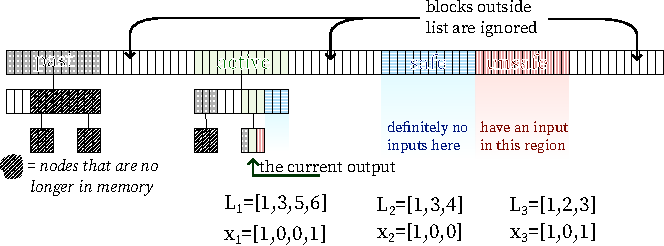
\includegraphics[width=15cm]{figures/rt-alg.pdf}
  \caption{Diagram showing the state of the algorithm in \Cref{alg:rt} and how it relates to the parts of the implicit random tree that the algorithm traverses. Positions on the horizontal axis correspond to different integers in $[n]$. To keep the example legible, we set parameters $d = 3$,  $w_1 = 7, w_2 = 4, w_3 = 3$, and $b_1 = 4, b_2 = 3, b_3 = 3$. \label{fig:rt-ub-intuition}}
\end{figure}

In order to prove that the algorithm in \Cref{alg:rt} is correct, we will need some additional notation. Let $d,\alpha,b_1,\ldots,b_d,w_1,\ldots,w_d$ be
as defined in \Cref{alg:rt}. It is helpful to view this algorithm as traversing over the leaves of a random tree of height $d$, in which:
\begin{itemize}
  \item Every node $v$ in the tree is associated with a subset $S_v$ of $[n]$. We say a node is at level $i$ if it is at depth $i - 1$. All nodes at a given level have disjoint associated subsets.
  \item The ``root'' $\rho$ of the tree has $S_\rho$ of size $\prod_{i=1}^{d} w_i$, and is at level $1$
  \item Each node $v$ at level $i$ (depth $i-1$) has $b_{i+1}$ children; the set $S_v$ is partitioned into $w_{i+1}$ parts of equal size, and each child of $v$ is associated with a random and unique one of these parts
  \item Each leaf node $u$, at depth $d$, is associated with a set of size 1, i.e., a single and unique integer in $[n]$. There are $\prod_{i=1}^{d} b_i$ leaf nodes in total.
\end{itemize}
See for example \Cref{fig:rt-ub-intuition}. The algorithm maintains a view of just the branch of the tree from the root to the current leaf node. Its output will be the number associated to this leaf. For each node $v$ on this branch, at level $i \in [d]$ (depth $i-1$), it keeps a record of the positions $L_i \in [w_i]^{b_i}$ of its children, and a record $x_i \in \{0,1\}^{b_i}$ indicating their status. There are four categories for child nodes:
\begin{itemize}
\item A node is \textsc{past} if the traversal over the tree passed through and leaf the node; past nodes are marked with a $1$ in $x_i$.
\item A node is \textsc{active} if it is on the branch to the current leaf node; this is the node with the lowest index which is marked with a $0$ in $x_i$.
\item A node $v$ is \textsc{safe} if it comes after the active node, and the adversary has never sent an input in $S_v$; safe nodes are marked with a $0$ in $x_i$.
\item A node $v$ is \textsc{unsafe} if it comes after the active node, and the adversary did send an input in $S_v$; unsafe nodes are marked with a $1$ in $x_i$.
\end{itemize}
The algorithm maintains these records as the adversary sends new inputs,
marking safe child nodes $v$ as unsafe if an element in $S_v$ is received. The
current leaf node is found by, from the root, following the chain of active
nodes. If the adversary sends the value of the current leaf node, the
algorithm will mark it by setting the corresponding entry in $x_d$ to $1$,
thereby changing the value of the current active node. If every element of
$x_d$ is a now $1$, this means that the adversary has sent an input for every
child of the level $d$ node on the current branch, so the algorithm marks the
current active child of the level $d - 1$ node with a $1$, thereby moving the
current branch to use a new level $d$ node, $u$, which is
\emph{safe}.\footnote{If the level $d - 1$ node has no children marked with a
$0$ after this, we repeat the process at level $d -2$, and so on.} It the
``loads the positions of the children of $u$''---the tree being randomly
generated, this is implemented by $L_d$ being randomly sampled and $x_d$ being
reset to be all zeros---and proceeds.

While there are $\prod_{i=1}^{d} b_i$ leaf nodes in the ideal random tree, the algorithm's traversal of them may skip a fraction, because they (or one of their ancestors) were marked as unsafe. We say that such leaf nodes, along with those which were once active, have been \textsc{killed}.


\begin{algorithm}
  \caption{Adversarially robust random tape algorithm for $\mif(n,\rl)$ with error $\le \delta$}
  \label[listing]{alg:rt}

  \begin{algorithmic}[1]
  \Statex Requirements: $\rl \le n / 64$ and $\rl \ge 4$.
  \Statex Parameters: $d = \min(\ceil{\log \rl}, \floor{2 \frac{\log(n/4)}{\log 16 \rl}})$. % ell: number of layers, is >= 2 always
  \Statex $\alpha = \begin{cases}2 & \text{if $\ceil{\log \rl} <  \floor{2 \frac{\log(n/4)}{\log 16 \rl}}$} \\ \frac{(4 \rl)^{2/(d-1)}}{(n/4)^{2/(d(d-1))}} & \text{otherwise}\end{cases}$
    \Statex Let $u$ be chosen via \Cref{lem:fract-power-round}, so that $\alpha^{d-2} \le \prod_{i=2}^{d-1} b_i \le 2 \alpha^{d-2}$
    \Statex $b_2 = \ldots = b_u = \ceil{\alpha}$, and $b_{u+1} = \ldots = b_{d-1} = \floor{\alpha}$
    \Statex $b_1 = \min(\rl + 1, \ceil{8 \alpha} + \ceil{3 \log 1/\delta})$; and $b_d = \ceil{ \frac{\rl}{\alpha^{d-1}} }$
    \Statex $w_1 = 16 \rl$; and for each $i \in \{2, \ldots, d\}$, $w_i = \prod_{j=i}^{d} b_j$.
  
  \Statex Let $\iota : [w_1]\times[w_2]\times \cdots \times [w_d] \rightarrow [n]$ be an arbitrary injective function
  
  \Statex
  \Statex \ul{\textbf{Initialization}}:
    \For{$i \in [d]$}
      \State $L_i \gets $ random sequence without repetition in $[w_i]^{b_i}$
      \State $x_i \gets (0,\ldots,0) \in \{0,1\}^{b_i}$
    \EndFor
    
  \Statex
  \Statex \ul{\textbf{Update}($a \in [n]$)}: % -> result
    \If{ $a \notin \iota^{-1}[n]$ } \textbf{return} \Comment{Any integer not in $\iota^{-1}[n]$ can never be an output}\EndIf
    \State $v_1,\ldots,v_d = \iota^{-1}(a)$ \Comment{Map input into $[w_1]\times\ldots\times[w_d]$}
    \State For $i \in [d]$, define $c_i = \min |\{j : x_i[j] = 0\}|$
    
    \If{for all $i\in[d]$, $v_i = L_i[c_i]$}
        \LineComment{Move to the next leaf node, sampling new child node positions as necessary}
        \For{$i = d,\ldots,1$}
          \State $x_i[c_i] \gets 1$
          \If{$x_i$ is the all-1s vector}
            \If{$i = 1$} \textbf{abort}  \Comment{If we reach $i=1$, then even the root node is full}\EndIf
            \State $L_i \gets $ random sequence without repetition in $[w_i]^{b_i}$
            \State $x_i \gets (0,\ldots,0)$
          \Else \ \textbf{break}
          \EndIf
        \EndFor
    \Else
        \LineComment{Mark a branch as unsafe, if there was a hit}
        % convert to for loop?
        \State Let $j$ be the smallest integer in $[d]$ for which $v_j \ne L_{j}[c_j]$. 
        \If{$\exists y \in [b_j]$ for which $L_j[y] = v_j$}
            \State $x_j[y] \gets 1$
        \EndIf
    \EndIf
    
  \Statex
  \Statex \ul{\textbf{Output} $\rightarrow [n]$}:
    \State For $i \in [d]$, define $c_i = \min |\{j : x_i[j] = 0\}|$
    \State \textbf{return} $\iota[ (L_1[c_1],L_2[c_2],\ldots,L_d[c_d]) ]$
  \end{algorithmic}
  
\end{algorithm}

\Cref{alg:rt} uses the following lemma to set some of its parameters; the specific rounding scheme for the values $b_2,\ldots,b_{d-1}$ ensures that $b_1$ can
decrease relatively smoothly as $\rl$ decreases. (Setting all $b_2=\ldots=b_{d -1}$ to $\floor{\alpha}$ can lead to having $b_1$ be significantly larger than
necessary (by up to a factor $(3/2)^d = \rl^{O(1)}$); setting all $b_2=\ldots=b_{d -1}$ to $\ceil{\alpha}$ would violate the $\prod_{i=1}^{d} w_i \le n$ constraint.)

\begin{lemma}\label{lem:fract-power-round}
  Let $\alpha \ge 1$. Then for all $k \ge 0$, there exists an integer $u$ depending
  on $\alpha$ and $k$ so that 
  \begin{align*}
    \alpha^k \le \ceil{\alpha}^u \floor{\alpha}^{k - u} \le 2 \alpha^k \,.
  \end{align*}
\end{lemma}

\begin{proof}[Proof of \Cref{lem:fract-power-round}]
  If $\alpha$ is an integer, we are done. Otherwise, with
  \begin{align*}
    u = \ceil{\frac{k \log(\alpha/\floor{\alpha})}{\log(\ceil{\alpha} /\floor{\alpha})}} \,, \quad \text{we have} \quad \ceil{\alpha}^u \floor{\alpha}^{k - u} = \floor{\alpha}^{k} (\ceil{\alpha}/\floor{\alpha})^u \ge \floor{\alpha}^{k} (\ceil{\alpha/\floor{\alpha}})^k = \alpha^k \,.
  \end{align*}
  Similarly, $\ceil{\alpha}^u \floor{\alpha}^{k - u} \le \alpha^k \ceil{\alpha}/\floor{\alpha}$, which is $\le 2\alpha^k$ because $\alpha \ge 1$ implies $\ceil{\alpha}/\floor{\alpha} \le 2$.
\end{proof}

The following lemma is straightforward but tedious, and we defer its proof to  \Cref{subsec:rt-ub-mech}.

\begin{lemma}\label{lem:rt-alg-params}
  The parameters of \Cref{alg:rt} satisfy the following conditions:
  \begin{align}
      \prod_{i=2}^{d} b_i &\ge \frac{\rl}{\alpha} \,, \label{eq:rt-ub-param-ge-l} \\
      \prod_{i=2}^{d} b_i &\le \frac{4 \rl}{\alpha} \,, \label{eq:rt-ub-param-le-2l}\\
      \prod_{i \in [d]} w_i &\le n \,. \label{eq:rt-ub-param-le-n}
  \end{align}
\end{lemma}

We now prove the main lemma:

\begin{lemma}\label{lem:rt-ub-error-limit}
  \Cref{alg:rt} has error $\le \delta$ in the adversarial setting.
\end{lemma}

\begin{proof}[Proof of \Cref{lem:rt-ub-error-limit}]
  We prove, using a charging scheme, that the probability of all leaf nodes
  in the random tree traversed by the algorithm being killed is $\le \delta$.

  The input of the adversary at any step falls into one of $d + 2$ categories.
  For each $i \in [d]$, it could add an input which intersects the list
  of unrevealed child positions of the level $i$ node, possibly killing
  $\prod_{j=i + 1}^{d} b_i$ leaf nodes if it guesses correctly. It could
  also send the value of the current leaf 
  node, thereby killing it (and only it).
  Finally, the adversary's input could be entirely wasted (outside $\iota([w_1]\times\ldots\times[w_d]$, repeating an input it made before, or in
  the region corresponding to one of the past nodes in the random tree); then
  no leaf nodes would be killed.

  As the algorithm proceeds, for each node in the random tree (other than
  the root), we accumulate charge. When the algorithm's current branch changes
  to use new nodes, the charge on the old nodes is kept, and the new nodes
  start at charge $0$.
  
  When the adversary makes an input that is handled by level $i$ ("query" at level $i$),
  for $i \in \{2,\ldots,d\}$, it
  \emph{first} deposits one unit of charge at the active level $i$ node.
  Then, if the query was a hit (i.e, ruled out some future subtree and made
  a child of a node in the current branch change from ``safe'' to ``unsafe''), increase
  the number of killed nodes by the number of leaves for the subtree
  (namely, $\prod_{j={i+1}}^{d} b_j$), and remove up to that amount 
  of charge from the node. The definitions of $(w_j)_{j=2,\ldots,d}$ ensure
  that $\prod_{j={i+1}}^{d} b_j = w_j / b_j$.
  
  For the $t$th query, let $K_t$ be the number of killed leaf nodes on the query,
  minus any accumulated charge on the node. Say the adversary picks a node at level $i$ for $i \in \{2,\ldots,d-1\}$, and that
  node has $\hw$ unexplored subtree regions (i.e, neither revealed because
  the algorithm produced outputs in them, nor because there was there a query at that subtree region
  in the past), and $\hb$ gives the number of subtrees within this unexplored
  region. If $\hb = 0$, $\EE[K_t | K_1,\ldots,K_{t-1}] = 0$. Otherwise, let $u$ be the number of subtrees which were revealed by the algorithm so far; we have $\hw \le w_j - u$ and $\hb \le b_j - u$. Then when we condition on the past increases in charge, the subtree regions within the unexplored region are still uniformly random; hence
  the probability of hitting a subtree is $\hb / \hw$. The number of leaf nodes
  killed by a hit is $w_j / b_j$.  The total charge currently at the node must be
  $\ge (w_j - u - \hw) - (\frac{w_j}{b_j}) (b_j - u - \hb) = \hb \frac{w_j}{b_j} - \hw + (\frac{w_j}{b_j} - 1) u \ge \hb \frac{w_j}{b_j} - \hw$, since each removed node consumes at most $\frac{w_j}{b_j}$ of the existing charge.
  Consequently, the increase in killed leaf nodes if we hit is $\max(0, \frac{w_j}{b_j} - \max(0, \hb \frac{w_j}{b_j} - \hw))$, so the expected payoff is\footnote{When the level is $d$ and $b_j=w_j$, we in fact we have $K_t = 1$ always; but we do not need this stronger fact.}:
  \begin{align*}
    \EE[K_t \mid K_1,\ldots,K_{t-1}] = \frac{\hb}{\hw} \max\left(0,\, \frac{w_j}{b_j} - \max\left(0,\, \hb \frac{w_j}{b_j} - \hw\right)\right) \underset{\text{by \Cref{lem:charge-adjusted-gain}}}{\le} 1 \,.
  \end{align*}
  
  If the level is $1$, then let $J \subseteq [16 \rl]$ give the set of probed subtree positions,
  and $H$ give the set of revealed subtree positions; since there are $\le \rl$ queries,
  $|J|,|H|$ are both $\le \rl$, and the probability of a query in an unexplored
  region to hit is $\le \frac{b_1}{16 \rl - |J \cup H|} \le \frac{b_1}{14 \rl}$. The charging scheme does not apply, so
  \begin{align*}
    \EE[K_t \mid K_1,\ldots,K_{t-1}] \le \frac{b_1}{14 \rl} \cdot \prod_{j=2}^{d} b_j \,.
    %\le \frac{b_1}{14 \rl} \cdot \frac{4 \rl}{\alpha} = \frac{2 b_1}{7 \alpha}
  \end{align*}
  
  Thus in all cases, $\EE[K_t \mid K_1,\ldots,K_{t-1}] \le \max(1,\, \prod_{j=1}^{d} b_j / 14 \rl)$. 
  
  The total charge deposited on mid-level nodes is $\le \rl$. The algorithm is guaranteed to succeed if the total number of leaves killed is less than the total number of leaves; i.e, if $\sum_{i \in [\rl]} K_t + \rl \le \prod_{j=1}^{d} b_j$. Note that by \Cref{lem:rt-alg-params} and the definition of $b_1$, $\prod_{j=1}^{d} b_j \ge b_1 \rl / \alpha \ge 8 \rl$. Consequently,
  \begin{align*}
    \rl + 7 \EE\left[\sum_{t = 1}^{\rl} K_t\right] 
    \le 8 \max\left(\rl,\, \frac{1}{14} \prod_{j=1}^{d} b_j\right)
    \le 8 \max\left(\frac{1}{8},\, \frac{1}{14}\right) \prod_{j=1}^{d} b_j \le  \prod_{j=1}^{d} b_j \,.
  \end{align*}
  Now let $D_t = K_t / \prod_{j=2}^{d} b_j$, so that each $D_t \in [0,1]$. Writing events in terms of $D_t$ lets us use \Cref{lem:azumanoff} to bound the probability that too many leaves are killed:
  \begin{align*}
  \Pr\left[\rl + \sum_{t \in [\rl]} K_t \ge \prod_{i=1}^{d} b_i\right] &\le 
      \Pr\left[\sum_{t \in [\rl]} K_t \ge 7 \max\Big(\rl, \frac{1}{14} \prod_{j=1}^{d} b_j\Big) \right] \\
      &\le \Pr\left[\sum_{t \in [\rl]} D_t \ge 7 \max\Big(\rl / \prod_{j=2}^{d} b_j, \frac{b_1}{14} \Big) \right] \\
      &\le \exp\left( - \frac{6^2}{2+6} \max\Big(\rl / \prod_{j=2}^{d} b_j, \frac{b_1}{14} \Big) \right) \\
      &\le \exp\left( - \frac{9 b_1}{28} \right) \le 2^{b_1 \cdot \frac{9}{28 \ln 2}} \le 2^{\ceil{3 \log 1/\delta} \frac{9}{28 \ln 2}} \le \delta \,. \qedhere
  \end{align*}  
\end{proof}

In the preceding proof, we used the following:

\begin{lemma}\label{lem:charge-adjusted-gain}
  Let $\hb,\hw,b,w$ be positive, and $\hb \ge 1$. Then:
  \begin{align*}
    \frac{\hb}{\hw} \left( \max\left(0,\, \frac{w}{b} - \max\left(\hb \frac{w}{b} - \hw,\, 0\right) \right)\right) \le 1 \,.
  \end{align*}
\end{lemma}

\begin{proof}[Proof of \Cref{lem:charge-adjusted-gain}]
  If $\frac{\hb}{\hw} \le \frac{b}{w}$, then:
  \begin{align*}
    \frac{\hb}{\hw} \left( \max(0, \frac{w}{b} - \max(\hb \frac{w}{b} - \hw, 0) )\right) \le \frac{\hb}{\hw} \frac{w}{b} \le 1 \,.
  \end{align*}
  Otherwise, $\frac{\hb}{\hw} \ge \frac{b}{w}$, and:
  \begin{align*}
    \frac{\hb}{\hw} &\left( \max\left(0,\, \frac{w}{b} - \max\left(\hb \frac{w}{b} - \hw,\, 0\right) \right)\right) \\
      &\le \frac{\hb}{\hw} \left(\frac{w}{b} - \left(\hb \frac{w}{b} - \hw\right)\right) 
      = \frac{\hb}{\hw} \left(\frac{w}{b} - \hb \left(\frac{w}{b} - \frac{\hw}{\hb}\right)\right)\\
      &\le \frac{\hb}{\hw} \left(\frac{w}{b} - 1 \left(\frac{w}{b} - \frac{\hw}{\hb}\right)\right) = \frac{\hb}{\hw} \frac{\hw}{\hb} = 1 \,, \qquad\quad \text{since $\hb \ge 1$ and $\frac{w}{b} - \frac{\hw}{\hb} \ge 0$ \,.} \qedhere
  \end{align*}
\end{proof}


The proof of the following lemma is a mostly straightforward calculation, which we defer to \Cref{subsec:rt-ub-mech}.

\begin{lemma}\label{lem:rt-ub-space-usage}
  \Cref{alg:rt} uses 
  \begin{align}
    O\left(\ceil{\frac{(4 \rl)^{2/(d-1)}}{(n/4)^{2/(d(d-1))}}} (\log \rl)^2 + \min(\rl, \log 1/\delta) \log \rl \right) \label{eq:rt-ub-semiprec-space}
  \end{align} bits of space, where $d = \min\left(\ceil{\log \rl}, \floor{2 \frac{\log(n/4)}{\log(16\rl)}}\right)$. A weaker upper bound on this is:
  \begin{align*}
    O\left(\rl^{\frac{\log \rl}{\log n}} (\log \rl)^2 + \min(\rl, \log 1/\delta) \log \rl\right) \,.
  \end{align*}
\end{lemma}


If $\rl \ge 4$ and $\rl \le n/64$, then \Cref{lem:rt-ub-space-usage} and \Cref{lem:rt-ub-error-limit} together show that \Cref{alg:rt} has error $\le \delta$ and space
usage as bounded by \cref{eq:rt-ub-semiprec-space}. To handle the cases where
$\rl < 4$ and $\rl > n/64$, one can instead use the simple deterministic algorithm
for $\mif(n,\rl)$ from \cite{Stoeckl23}, using only $\rl$ bits of space. As this is in
fact less than the space upper bound from \cref{eq:rt-ub-semiprec-space}, it follows
that \cref{eq:rt-ub-semiprec-space} gives an upper bound on the space
needed for a random tape, adversarially robust $\mif(n,\rl)$ algorithm for any
setting of parameters. Formally:


\begin{theorem} %{rtubintro}
\label{thm:rt-ub-intro}
  There is a family of adversarially robust random tape algorithms, where
  for $\mif(n,\rl)$ the corresponding algorithm has $\le \delta$ error and uses
  \begin{align*}
    O\left(\ceil{ 
    \frac{(4 \rl)^{\frac{2}{d - 1}}}{(n/4)^{\frac{2}{d(d-1)}}}
    } (\log \rl)^2 + \min(\rl,\, \log \tfrac{1}{\delta}) \log \rl \right)
  \end{align*}
  bits of space, where $d = \max\left(2, \min\left(\ceil{\log \rl}, \floor{2 \frac{\log(n/4)}{\log(16\rl)}}\right)\right)$. When $\delta = 1/\poly(n)$ a (weakened) space bound is $O\left(\rl^{\log_n \rl} (\log \rl)^2 + \log \rl\log n\right)$.
\end{theorem}

\subsection{Mechanical Proofs for \texorpdfstring{\Cref{sec:rt-ub}}{Random Tape Upper Bound}}\label{subsec:rt-ub-mech}

\begin{proof}[Proof of \Cref{lem:rt-alg-params}]
  First, we handle the case where $\ceil{\log \rl} <  \floor{2 \frac{\log(n/4)}{\log 16 \rl}}$. Then $d = \ceil{\log \rl} \le \floor{2 \frac{\log(n/4)}{\log 16 \rl}} - 1$, and $\alpha = 2$. Note that $\frac{\rl}{2^{d - 1}} \ge 1$ since $2^{d - 1} \le  2^{\ceil{\rl} - 1} \le 2\rl/2 = \rl$.
  \begin{align*}
      \prod_{i=2}^{d} b_i &= \ceil{\frac{\rl}{2^{d - 1}}} 2^{d - 2} \ge \frac{\rl}{2} = \frac{\rl}{\alpha} \\
      \prod_{i=2}^{d} b_i &=  \ceil{\frac{\rl}{2^{d - 1}}} 2^{d - 2} \le 2 \frac{\rl}{2} \le \frac{4 \rl}{\alpha} \,.
  \end{align*}
  Since $b_d = \ceil{\frac{\rl}{2^{d - 1}}} = \ceil{\frac{2 \rl}{2^{\ceil{\log \rl}}}} \le 2$,
  \begin{align*}
    \prod_{i \in [d]} w_i &= (16 \rl) \prod_{i = 2}^{d} \prod_{j=i}^{d} b_j
      \le (16 \rl) \prod_{i = 2}^{d} 2^{d - i + 1} = (16 \rl) 2^{d (d-1) / 2} \\
      &\le (16 \rl) (2^{\ceil{\log \rl}})^{(d-1) / 2} \le (16 \rl) (2 \rl)^{(d-1) / 2} \\
      &\le (16 \rl) (2 \rl)^{(\floor{2 \frac{\log (n/4)}{\log 16\rl}}-2) / 2} \\
      &\le (16 \rl) (2 \rl)^{\frac{\log (n/4)}{\log 16\rl} - 1} \\
      &\le (16 \rl)^{\frac{\log (n/4)}{\log 16\rl}} = \frac{n}{4} \le n \,.
  \end{align*}

  Second, we consider the case where $d = \floor{2 \frac{\log (n/4)}{\log(16\rl)}}$. Because $n \ge 64 \rl$, $d \ge 2$, and so
  \begin{align*}
    d = \floor{2 \frac{\log (n/4)}{\log 16 \rl}} \ge \frac{2}{3} \cdot 2 \frac{\log (n/4)}{\log 16 \rl} = \frac{\log (n/4)}{\frac{3}{4} \log 16 \rl} \ge \frac{\log (n / 4)}{\log 4 \rl} \,.
  \end{align*}
  The second inequality used that $\frac{3}{4} (4 + \log \rl) \le (2 + \log \rl)$ for $\rl \ge 4$. Consequently,
  \begin{align*}
    \alpha = \left(\frac{(4 \rl)^{d}}{n/4}\right)^{\frac{2}{d(d-1)}} \ge \left(\frac{(4 \rl)^{\frac{\log (n / 4)}{\log 4 \rl}}}{n/4}\right)^{\frac{2}{d(d-1)}} =  \left(\frac{n/4}{n/4}\right)^{\frac{2}{d(d-1)}} = 1 \,.
  \end{align*}
  We now prove Eq. \ref{eq:rt-ub-param-ge-l}. Because $\prod_{i=2}^{d-1} b_i \ge \alpha^{d - 2}$,
  \begin{align*}
    \prod_{i=2}^{d} b_i = \ceil{\frac{\rl}{\alpha^{d - 1}}} \prod_{i=2}^{d-1} b_i \ge \frac{\rl}{\alpha \prod_{i=2}^{d-1} b_i} \cdot \prod_{i=2}^{d-1} b_i = \frac{\rl}{\alpha} \,.
  \end{align*}
  For Eq. \ref{eq:rt-ub-param-le-n}, we observe that
  \begin{align*}
    d \le 2 \frac{\log(n/4)}{\log(16 \rl)}  \qquad \implies \qquad 16\rl \le (n/4)^{2/d} \qquad \implies \qquad \rl \ge \alpha^{d - 1} =\frac{(4 \rl)^2}{(n/4)^{2/d}} \,,
  \end{align*}
  and thus $\rl / \alpha^{d - 1} \ge 1$, so $b_d = \ceil{\rl / \alpha^{d -1}} \le 2 \rl / \alpha^{d - 1}$. Then since  $\prod_{i=2}^{d-1} b_i \le 2 \alpha^{d - 2}$,
  \begin{align*}
    \prod_{i=2}^{d} b_i \le \frac{2 \rl}{\alpha^{d - 1}} \prod_{i=2}^{d} b_i \le \frac{4 \rl}{\alpha \prod_{i=2}^{d-1} b_i} \cdot \prod_{i=2}^{d-1} b_i \le \frac{4 \rl}{\alpha} \,.
  \end{align*}
  Finally, we prove Eq. \ref{eq:rt-ub-param-le-n}. As noted above,
  \begin{align*}
    b_d \le \frac{2 \rl}{\alpha^{d-1}} \le \frac{4 \rl}{\alpha \prod_{i=2}^{d-1} b_j} \,.
  \end{align*}
  Applying this fact to bound the left hand side of Eq. \ref{eq:rt-ub-param-le-n} gives:
  \begin{align*}
    \prod_{i \in [d]} w_i &= (16 \rl) \prod_{i = 2}^d \prod_{j=i}^d b_j = 16 \rl (b_d)^d \prod_{i = 2}^{d-1} \prod_{j=i}^{d-1} b_j \\
      &\le 16 \rl \left(\frac{4 \rl}{\alpha \prod_{i=2}^{d-1} b_j} \right)^{d-1} \prod_{i = 2}^{d-1} \prod_{j=i}^{d-1} b_j \\
      &\le \frac{4 \cdot (4 \rl)^d}{\alpha^{d-1}} \frac{1}{\prod_{i = 2}^{d-1} \prod_{j=2}^{i-1} b_j} \\
      &\le \frac{4 \cdot(4 \rl)^d}{\alpha^{d-1}} \frac{1}{\alpha^{(d-1)(d-2)/2}} \qquad \text{since $\prod_{j=2}^{d-1} b_j \ge \alpha^{d-2}$ and $b_2 \ge b_3 \ge \ldots \ge b_{d-1}$} \\
      &= \frac{4 \cdot(4 \rl)^d}{\alpha^{d(d-1)/2}} = \frac{4 \cdot(4 \rl)^{d}}{\frac{(4 \rl)^d}{n / 4}} = n \,. \qedhere
  \end{align*}
\end{proof}




\begin{proof}[Proof of \Cref{lem:rt-ub-space-usage}]
  \Cref{alg:rt} only stores two types of data: for each $i\in[d]$, the vectors $L_i \in [w_i]^{b_i}$, and the vectors $x_i \in \{0,1\}^{b_i}$. These can be stored using $b_i \log w_i$ and $b_i$, bits respectively, for a total of:
  \begin{align*}
    \sum_{i \in [d]} b_i \log(2 w_i) &\le b_1 \log(2 w_1) + \sum_{i = 2}^{d} b_i \log(2 w_i) \\
      &\le b_1 \log(32 \rl) + \sum_{i = 2}^{d} b_i \log(2 \prod_{j=i}^{d} b_i)
      \le \sum_{i=1}^{d} b_i \log(32 \rl) \,,
  \end{align*}
  since by Eq. \ref{eq:rt-ub-param-le-2l}, $\prod_{j=i}^{d} b_i \le 4 \rl$. 
  
  We now observe that $b_d \le \ceil{\alpha}$. If $d = \ceil{\log \rl}$,
  then $\alpha = b_2 = \ldots = b_{d - 1} = 2$ and $b_d = \ceil{\rl/\alpha^{d - 1}} \le 2$. On the other hand, if $d = \floor{2 \frac{\log(n/4)}{\log(16\rl)}}$, then $\alpha = \frac{(4 \rl)^{2/(d-1)}}{(n/4)^{2/(d(d-1))}}$. We have:
  \begin{align*}
    (4\rl)^{d + 1} = (4\rl)^{\floor{2 \frac{\log(n/4)}{\log(16\rl)}} + 1} \ge (4\rl)^{2 \frac{\log(n/4)}{\log(16\rl)}} = (n/4)^2 \,,
  \end{align*}
  which implies
  \begin{align*}
    \alpha = \frac{(4 \rl)^{2/(d-1)}}{(n/4)^{2/(d(d-1))}} \ge \frac{(4 \rl)^{2/(d-1)}}{(4\rl)^{(d+1)/(d(d-1))}} = (4\rl)^{(2 - \frac{d+1}{d}) \cdot \frac{1}{d - 1}} = (4\rl)^{\frac{1}{d}} \,.
  \end{align*}
  Consequently,
  \begin{align*}
    b_d = \ceil{\frac{\rl}{\alpha^{d - 1}}} = \ceil{\frac{1}{4} \frac{4 \rl}{\alpha^{d - 1}}} \le \ceil{\frac{1}{4} (4 \rl)^{1/d}} \le (4 \rl)^{1/d} \le \alpha \,.
  \end{align*}
  
  With the bound on $b_d$, and the fact that $\alpha \ge 1$ in both cases, and that $d \le \ceil{\log \rl}$ we obtain:
  \begin{align*}
    \sum_{i \in [d]} b_i &\le \min(\rl + 1, \ceil{8 \alpha} + \ceil{3 \log 1/\delta}) + (d - 1) \ceil{\alpha} \\
      &\le \min(\rl, \ceil{3 \log 1/\delta}) + (7 + d) 2 \alpha \\
      &\le \min(\rl, \ceil{3 \log 1/\delta}) + 32 \log \rl \ceil{\frac{(4 \rl)^{2/(d-1)}}{(n/4)^{2/(d(d-1))}}} \,.
  \end{align*}
  Multiplying this last quantity by $\log(32 \rl)$ gives a space bound.

  To obtain a much weaker, but somewhat more comprehensible upper bound on $\alpha$, when $d = \floor{2 \frac{\log(n/4)}{\log(16\rl)}}$, we note that:
  \begin{align*}
    \max_{\lambda \in \NN \cap [2,\infty)} \log \frac{(4 \rl)^{2/(\lambda-1)}}{(n/4)^{2/(\lambda(\lambda-1))}} &\le \log \max_{\lambda \in \RR \cap [2,\infty)} \left(\frac{2}{\lambda - 1} \log(4\rl) - \frac{2}{\lambda(\lambda-1)} \log(n/4) \right) \\
    &\le \log \left(2 \log(4\rl) \max_{\lambda \in \RR \cap [2,\infty)} \left(\frac{1}{\lambda - 1} - \frac{1}{\lambda (\lambda -1)} \frac{\log(n/4)}{\log(4\rl)} \right)\right) \,.
  \end{align*}
  Let $\gamma = \frac{\log(n/4)}{\log(4\rl)}$; this is $\ge 1$. Let $f(x) = \frac{1}{x - 1} (1 - \frac{\gamma}{x})$. We will now prove that $\max_{x \ge 2} f(x) \le \frac{1}{2\gamma}$. We note that when $x = 2$, we have:
  \begin{align*}
    f(2) = 1 - \frac{\gamma}{2} \le \frac{1}{2\gamma} \,.
  \end{align*}
  Checking the other endpoint, we have:
  \begin{align*}
    \lim_{x \rightarrow \infty} \frac{1}{x - 1} (1 - \frac{\gamma}{x}) = 0 \,.
  \end{align*}
  Since $f(x)$ is differentiable on $[2,\infty)$, if it has a maximum other than at the endpoints, then it will occur when $\frac{d}{dx} f(x) = 0$. Solving this equation, we obtain:
  \begin{align*}
    \frac{d}{dx} f(x) = -\frac{1}{\left(x-1\right)^{2}}+\frac{\gamma\left(2x-1\right)}{\left(x\left(x-1\right)\right)^{2}} = -\frac{1}{\left(x-1\right)^{2}}\left[1-\frac{\gamma\left(2x-1\right)}{x^{2}}\right] = 0 \,,
  \end{align*}
  which is true iff $x^2 = \gamma(2x - 1)$. The solutions to the quadratic equation are
  \begin{align*}
    x = \gamma-\sqrt{\gamma\left(\gamma-1\right)} \qquad \text{and} \qquad  x = \gamma+\sqrt{\gamma\left(\gamma-1\right)} \,.
  \end{align*}
  Since $\gamma \ge 1$, the $-$ branch has $x \le 1$, which is not in $[2,\infty)$. The $+$ branch is only in $[2,\infty)$ if $\gamma \ge \frac{4}{3}$. The value of $f(x)$ in this case is:
  \begin{align*}
    f(\gamma+\sqrt{\gamma\left(\gamma-1\right)}) &= \frac{1}{\gamma+\sqrt{\gamma\left(\gamma-1\right)} - 1} \left(1 - \frac{\gamma}{\gamma+\sqrt{\gamma\left(\gamma-1\right)}} \right) \\
      &= \frac{\sqrt{\gamma(\gamma-1)}}{2 \gamma - 1 + 2 \sqrt{\gamma(\gamma-1)}} \\
      &\le \frac{1}{4 \sqrt{\gamma(\gamma-1)}}  &&\hspace{-4cm}\text{(since $\sqrt{\gamma(\gamma-1)} \le 2 \gamma - 1$ for all $\gamma \ge 1$)}
      \\
      &\le \frac{1}{2 \gamma} \,. &&\hspace{-4cm}\text{(since $\gamma \le 2 \sqrt{\gamma(\gamma-1)}$ for all $\gamma \ge \frac{4}{3}$)}
  \end{align*}
  Thus, if $f(x)$ does have a maximum in $[2,\infty)$, it is $\le \frac{1}{2\gamma}$. We conclude that $f(x) \le \frac{1}{2\gamma}$ in all cases. This proves:
  \begin{align*}
    \log \alpha \le \max_{\lambda \in \NN} \log \frac{(4 \rl)^{2/(\lambda-1)}}{(n/4)^{2/(\lambda(\lambda-1))}} 
      &\le \log\left(2 \log(4 \ell) \frac{1}{2 \frac{\log(n/4)}{\log(4\rl)}} \right) \le \log \frac{  \log(4 \ell)^2}{\log(n/4)} \,. \qedhere
  \end{align*}
\end{proof}

\newcommand{\etalchar}[1]{$^{#1}$}
\begin{thebibliography}{GGMW20}

\bibitem[ABJ{\etalchar{+}}22]{AjtaiBJSSWZ22}
Mikl\'os Ajtai, Vladimir Braverman, T.S. Jayram, Sandeep Silwal, Alec Sun,
  David~P. Woodruff, and Samson Zhou.
\newblock The white-box adversarial data stream model.
\newblock In {\em Proc. 41st ACM Symposium on Principles of Database Systems},
  pages 15--27, 2022.

\bibitem[ACGS23]{AssadiCGS23}
Sepehr Assadi, Amit Chakrabarti, Prantar Ghosh, and Manuel Stoeckl.
\newblock Coloring in graph streams via deterministic and adversarially robust
  algorithms.
\newblock In {\em Proc. 42nd ACM Symposium on Principles of Database Systems},
  pages 141--153, 2023.

\bibitem[BEEO22]{BenEliezerEO22}
Omri Ben-Eliezer, Talya Eden, and Krzysztof Onak.
\newblock Adversarially robust streaming via dense-sparse trade-offs.
\newblock In {\em Symposium on Simplicity in Algorithms (SOSA)}, pages
  214--227, 2022.

\bibitem[BJWY20]{BenEliezerJWY20}
Omri Ben{-}Eliezer, Rajesh Jayaram, David~P. Woodruff, and Eylon Yogev.
\newblock A framework for adversarially robust streaming algorithms.
\newblock In {\em Proc. 39th ACM Symposium on Principles of Database Systems},
  page 63–80, 2020.

\bibitem[BKKS23]{BravermanKKS23}
Vladimir Braverman, Robert Krauthgamer, Aditya Krishnan, and Shay Sapir.
\newblock Lower bounds for pseudo-deterministic counting in a stream.
\newblock {\em arXiv preprint arXiv:2303.16287}, 2023.

\bibitem[BR93]{BellareR93}
Mihir Bellare and Phillip Rogaway.
\newblock Random oracles are practical: A paradigm for designing efficient
  protocols.
\newblock In {\em Proc. 1st ACM Conference on Computer and Communications
  Security}, pages 62--73, 1993.

\bibitem[BY20]{BenEliezerY20}
Omri Ben{-}Eliezer and Eylon Yogev.
\newblock The adversarial robustness of sampling.
\newblock In {\em Proc. 39th ACM Symposium on Principles of Database Systems},
  pages 49--62. {ACM}, 2020.

\bibitem[CGS22]{ChakrabartiGS22}
Amit Chakrabarti, Prantar Ghosh, and Manuel Stoeckl.
\newblock Adversarially robust coloring for graph streams.
\newblock In {\em Proc. 13th Conference on Innovations in Theoretical Computer
  Science}, pages 37:1--37:23, 2022.

\bibitem[Fei19]{Feige19}
Uriel Feige.
\newblock A randomized strategy in the mirror game.
\newblock {\em arXiv preprint arXiv:1901.07809}, 2019.

\bibitem[GGMW20]{GoldwasserGMW20}
Shafi Goldwasser, Ofer Grossman, Sidhanth Mohanty, and David~P. Woodruff.
\newblock {Pseudo-Deterministic Streaming}.
\newblock In {\em Proc. 20th Conference on Innovations in Theoretical Computer
  Science}, volume 151, pages 79:1--79:25, 2020.

\bibitem[GGS23]{GrossmanGS23}
Ofer Grossman, Meghal Gupta, and Mark Sellke.
\newblock Tight space lower bound for pseudo-deterministic approximate
  counting.
\newblock {\em arXiv preprint arXiv:2304.01438}, 2023.

\bibitem[GS18]{GargS18}
Sumegha Garg and Jon Schneider.
\newblock {The Space Complexity of Mirror Games}.
\newblock In {\em Proc. 10th Conference on Innovations in Theoretical Computer
  Science}, pages 36:1--36:14, 2018.

\bibitem[HKM{\etalchar{+}}20]{HassidimKMMS20}
Avinatan Hassidim, Haim Kaplan, Yishay Mansour, Yossi Matias, and Uri Stemmer.
\newblock Adversarially robust streaming algorithms via differential privacy.
\newblock In {\em Advances in Neural Information Processing Systems 33: Annual
  Conference on Neural Information Processing Systems 2020, NeurIPS 2020,
  December 6-12, 2020, virtual}, 2020.

\bibitem[HW13]{HardtW13}
Moritz Hardt and David~P. Woodruff.
\newblock How robust are linear sketches to adaptive inputs?
\newblock In {\em Proc. 45th Annual ACM Symposium on the Theory of Computing},
  pages 121--130, 2013.

\bibitem[Ind06]{Indyk06}
Piotr Indyk.
\newblock Stable distributions, pseudorandom generators, embeddings, and data
  stream computation.
\newblock {\em J. ACM}, 53(3):307--323, 2006.

\bibitem[JP83]{JoagDevP83}
Kumar {Joag-Dev} and Frank Proschan.
\newblock Negative association of random variables, with applications.
\newblock {\em Ann. Stat.}, 11(1):286--295, 1983.

\bibitem[JW23]{JayaramW23}
Rajesh Jayaram and David~P Woodruff.
\newblock Towards optimal moment estimation in streaming and distributed
  models.
\newblock {\em ACM Trans. Alg.}, 19(3):1--35, 2023.

\bibitem[KMNS21]{KaplanMNS21}
Haim Kaplan, Yishay Mansour, Kobbi Nissim, and Uri Stemmer.
\newblock Separating adaptive streaming from oblivious streaming using the
  bounded storage model.
\newblock In {\em Advances in Cryptology - {CRYPTO} 2021 - 41st Annual
  International Cryptology Conference, {CRYPTO} 2021, Virtual Event, August
  16-20, 2021, Proceedings, Part {III}}, volume 12827 of {\em Lecture Notes in
  Computer Science}, pages 94--121. Springer, 2021.

\bibitem[MN22a]{MagenN22}
Roey Magen and Moni Naor.
\newblock Mirror games against an open book player.
\newblock In {\em 11th International Conference on Fun with Algorithms (FUN
  2022)}, volume 226, pages 20:1--20:12, 2022.

\bibitem[MN22b]{MenuhinN22}
Boaz Menuhin and Moni Naor.
\newblock Keep that card in mind: Card guessing with limited memory.
\newblock In {\em Proc. 13th Conference on Innovations in Theoretical Computer
  Science}, pages 107:1--107:28, 2022.

\bibitem[New91]{Newman91}
Ilan Newman.
\newblock Private vs.~common random bits in communication complexity.
\newblock {\em Inform. Process. Lett.}, 39(2):67--71, 1991.

\bibitem[Nis90]{Nisan90}
Noam Nisan.
\newblock Pseudorandom generators for space-bounded computation.
\newblock In {\em Proc. 22nd Annual ACM Symposium on the Theory of Computing},
  pages 204--212, 1990.

\bibitem[Nis93]{Nisan93B}
Noam Nisan.
\newblock On read once vs. multiple access to randomness in logspace.
\newblock {\em Theoretical Computer Science}, 107(1):135--144, 1993.

\bibitem[Sto23]{Stoeckl23}
Manuel Stoeckl.
\newblock Streaming algorithms for the missing item finding problem.
\newblock In {\em Proc. 34th Annual ACM-SIAM Symposium on Discrete Algorithms},
  pages 793--818, 2023.
\newblock Full version at arXiv:2211.05170v1.

\bibitem[WZ22]{WoodruffZ22}
David~P. Woodruff and Samson Zhou.
\newblock Tight bounds for adversarially robust streams and sliding windows via
  difference estimators.
\newblock In {\em Proc. 62nd Annual IEEE Symposium on Foundations of Computer
  Science}, pages 1183--1196, 2022.

\end{thebibliography}
\end{document}
